\documentclass[nobib]{tufte-handout}

%\\geometry{showframe}% for debugging purposes -- displays the margins

\newcommand{\bra}[1]{\left(#1\right)}
\usepackage{hyperref}
\usepackage[activate={true,nocompatibility},final,tracking=true,kerning=true,spacing=true,factor=1100,stretch=10,shrink=10]{microtype}
\usepackage{color}

% Fixes captions and images being cut off
\usepackage{marginfix}
\usepackage{mdframed}
\usepackage{xcolor}
\usepackage{pgfplots}
\usepackage[americancurrents, americaninductors, americanvoltages, americanresistors]{circuitikz}
\usepackage{siunitx}
\usepackage{amsmath,amsthm}
\usepackage{circuitikz}
\usetikzlibrary{shapes}
\usetikzlibrary{positioning}
\usetikzlibrary{arrows}

% Set up the images/graphics package
\usepackage{graphicx}
\setkeys{Gin}{width=\linewidth,totalheight=\textheight,keepaspectratio}
\graphicspath{{.}}


\newmdenv[
    backgroundcolor=black!10, % Light blue shading inside the box
    linecolor=black,         % Border color
    linewidth=1pt,          % Border thickness
    roundcorner=5pt,        % Rounded corners
    skipabove=10pt,         % Space above the box
    skipbelow=10pt,         % Space below the box
    innertopmargin=5pt,     % Inner top margin
    innerbottommargin=5pt,  % Inner bottom margin
    innerleftmargin=10pt,   % Inner left margin
    innerrightmargin=10pt   % Inner right margin
]{defbox}

\title{Notes for ECE 45600 - Integrated Circuit Design}
\author[Shubham Saluja Kumar Agarwal]{Shubham Saluja Kumar Agarwal}
\date{\today}  % if the \date{} command is left out, the current date will be used

% The following package makes prettier tables.  We're all about the bling!
\usepackage{booktabs}

% The fancyvrb package lets us customize the formatting of verbatim
% environments.  We use a slightly smaller font.
\usepackage{fancyvrb}
\fvset{fontsize=\normalsize}

% Small sections of multiple columns
\usepackage{multicol}

% These commands are used to pretty-print LaTeX commands
\newcommand{\doccmd}[1]{\texttt{\textbackslash#1}}% command name -- adds backslash automatically
\newcommand{\docopt}[1]{\ensuremath{\langle}\textrm{\textit{#1}}\ensuremath{\rangle}}% optional command argument
\newcommand{\docarg}[1]{\textrm{\textit{#1}}}% (required) command argument
\newenvironment{docspec}{\begin{quote}\noindent}{\end{quote}}% command specification environment
\newcommand{\docenv}[1]{\textsf{#1}}% environment name
\newcommand{\docpkg}[1]{\texttt{#1}}% package name
\newcommand{\doccls}[1]{\texttt{#1}}% document class name
\newcommand{\docclsopt}[1]{\texttt{#1}}% document class option name

% Define a custom command for definitions
\newcommand{\defn}[2]{\noindent\textbf{#1}:\ #2}

\begin{document}

\maketitle

\begin{abstract}
    These are lecture notes for Fall 2025 ECE 45600 by professor Saeed Mohammadi at Purdue. Modify, use, and distribute as you please.
\end{abstract}

\tableofcontents

\newpage

\section{Noise and Reliability}
Noise in circuits comes from undesired coupling, both capacitive and
inductive.\\
\begin{mdframed}
    Note: Capacitive and inductive coupling are reduced by:
    \begin{itemize}
        \item Placing interconnected lines far from each other.
        \item Adding ground plane between lines.
        \item Reducing length of interconnected lines
    \end{itemize}
\end{mdframed}
The following is the graph of the voltage transfer characteristics of an inverter:
\begin{center}
    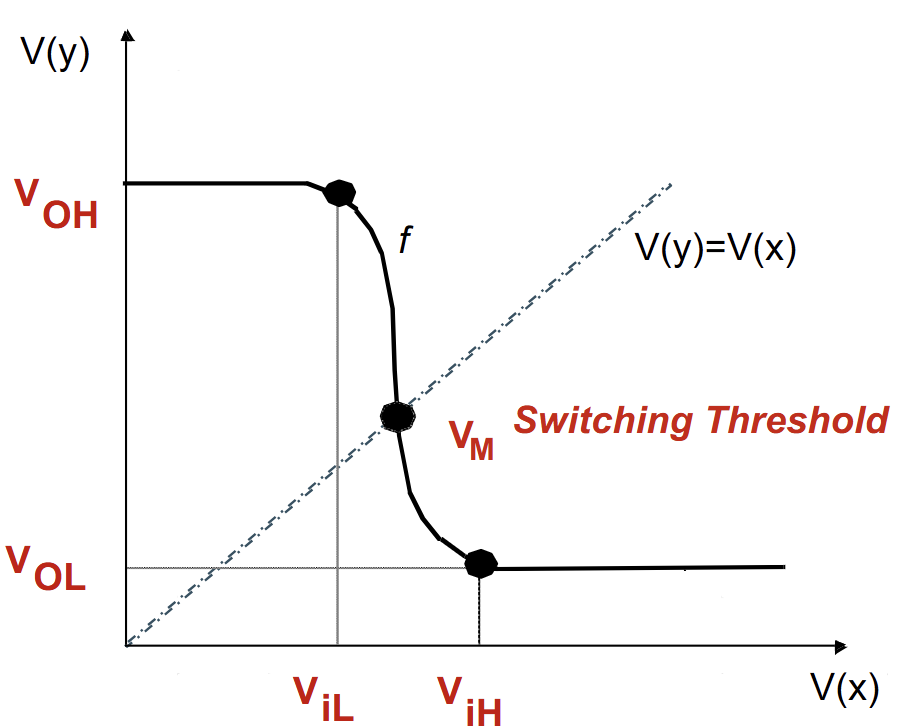
\includegraphics[width = 175px]{images/voltage_transfer_characteristics.png}
\end{center}
In it, $V_{OH} = f(V_{iH})$ is the voltage recognized as the output voltage when the inverter begins to output high. Similarly, $V_{OL} = f(V_{iL})$ is the voltage when it begins to output low. Finally, $V_M = f(V_M)$ is the point that the input and the output are the same, and is also known as the switching threshold.\\
Both $V_{iL}$ and $V_{iH}$ are points at which the curve has a slope of $-1$. The area between these two points is the undefined region, and is the reason why noise is a problem.\\
The range between the output and the input on each side of the curve is known as the noise margin, and is an area where the output is well defined into one of its two possible values:
\begin{center}
    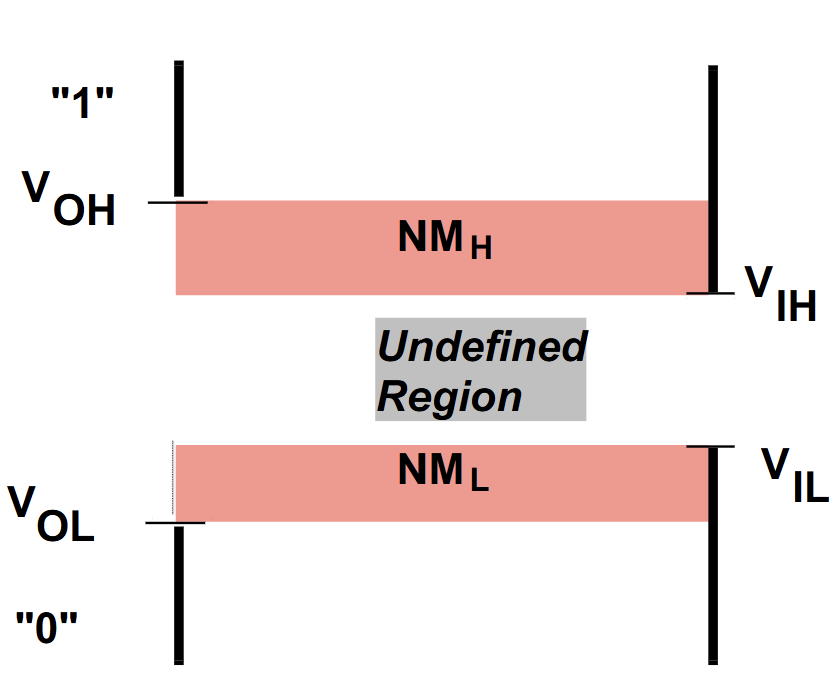
\includegraphics[width = 150px]{images/noise_margin.png}
\end{center}
There are two kinds of noise sources:
\begin{enumerate}
    \item Fixed Sources
    \item Proportional Sources
\end{enumerate}
The noise margin, $V_{NM}$, has the following properties:
\begin{equation*}
    \frac{V_{SW}}{2} \geq V_{NM}\geq \sum f_i V_{Nfi}+ \sum g_j V_{SW}
\end{equation*}
where $V_Nfi$ is a fixed noise source and $V_{SW}$ is a proportional one.\\
Noise margins are deceptive, as these can be easily disturbed, which is why the more reliable parameter is noise immunity, or the ability to suppress noise.
\begin{center}
    \includegraphics*[width = 200px]{images/noise_immunity.png}
\end{center}
The higher the impedance of the noise immunity, the more noise is rejected.\\
\subsection{Regenarative vs Non-Regenarative}
The following is a graph of a regenerative curve:
\begin{center}
    \includegraphics*[width = 150px]{images/regenerative_curve.png}
\end{center}
The behavior of this kind of curve is the following:\\
\textit{Let us imagine several inverters connected to each other in series. If the input voltage of the first inverter starts somewhere close to the center of the undefined region, after a few inverters, the output will be well into the noise margins.}\\
On the other hand, a non-regenerative curve,
\begin{center}
    \includegraphics*[width = 150px]{images/non_regenerative_curve.png}
\end{center}
\textit{In a series arrangement of inverters, if the input of one is undefined, the eventual inputs and outputs will tend to the center of the undefined region instead.}\\
This is why a regenerative curve is what we desire form our inverters.\\
\section{Fan-in and Fan-out}
We will now define two important terms in the context of gates:
\begin{multicols}{2}
    \begin{defbox}
        The fan-in is the number of inputs a gate has, and is represented by the letter $M$:
        \begin{center}
            \includegraphics*[width = 100px]{images/fanin.png}
        \end{center}
    \end{defbox}
    \begin{defbox}
        The fan-out is the number of outputs a gate has, and is represented by the letter $N$:
        \begin{center}
            \includegraphics*[width = 70px]{images/fanout.png}
        \end{center}
    \end{defbox}
\end{multicols}
\section{Gate Delays}
Another important gate parameter is the delay it possesses.  The delay of a gate will define how fast the circuit can run, as well as some restraints it will have to avoid errors.\\
This delay, as well as its subcomponents can be seen in the following figure:
\begin{center}
    \includegraphics*[width = 200px]{images/inverter_delay_plot.png}
\end{center}
In this image, we can see a few kinds of delays:
\begin{itemize}
    \item Fall delay $t_f$: the time it takes for the output curve to go from $V_{OH}$ to $V_{OL}$. Depends on the strength of the driver and the load presented to it.
    \item Fall delay $t_r$: the time it takes for the output curve to go from $V_{OL}$ to $V_{OH}$. Depends on the strength of the driver and the load presented to it.
    \item High to Low Propagation delay $t_{pHL}$: the time between the 50\% of the input to the 50\% voltage of the output when the inverter output is transitioning from high to low.
    \item Low to High Propagation delay $t_{pLH}$: the time between the 50\% of the input to the 50\% voltage of the output when the inverter output is transitioning from low to high.
    \item Propagation delay $t_p$: $(t_{pLH}+t_{pHL})/2$
\end{itemize}
Now, let us imagine the following circuit:
\begin{center}
    \includegraphics*[width = 200px]{images/inverter_cycle.png}
\end{center}
The input of the first inverter will be bouncing between high and low at a certain frequency, and thus we can deduce the propagation delay using the following formula:
\begin{equation*}
    T = 2 \times t_p \times N
\end{equation*}
\section{Inverter Modelling}
We can use an RC circuit to model the delay of an inverter as shown below:
\begin{center}
    \includegraphics*[width = 120px]{images/rc_inverter_delay.png}
\end{center}
This will work if the following two properties, brought about by their definitions withing the delay curve and the voltage transfer characteristics curve, hold true:
\begin{eqnarray*}
    t_p = \ln(2)\tau\\
    t_r \approx t_f = \ln(9)\tau
\end{eqnarray*}
\subsection{Power Dissipation}

\end{document}
